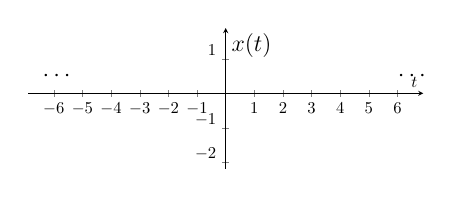
\begin{tikzpicture}[scale=0.6]
    \begin{axis}[
        x=.05\textwidth,y=0.06\textwidth,
    	axis y line=center,
    	axis x line=middle,
    	xlabel=$t$,ylabel={\Large $x(t)$},
    	xmin=-6.9,xmax=6.9,
    	ymin=-2.2,ymax=1.9,
    	xtick={-6,...,6},
    	xticklabel style = {xshift=0},
    	yticklabel style = {yshift=5}
	] 
	\diracdelta{-5}{-2};
	\diracdelta{-4}{1};
	\diracdelta{-3}{-2};
	\diracdelta{-2}{1};
	\diracdelta{-1}{-2};
	\diracdelta{0}{1};
	\diracdelta{1}{-2};
	\diracdelta{2}{1};
	\diracdelta{3}{-2};
	\diracdelta{4}{1};
	\diracdelta{5}{-2};
	\node at (axis cs:6.5,.5) {\Large $\cdots$} ;
	\node at (axis cs:-5.9,.5) {\Large $\cdots$} ;
    \end{axis}
\end{tikzpicture}